\bexo
Tracer sur la même figure
\begin{itemize}
	\item $x\mapsto \cos(x)$
	\item $x\mapsto \cos(2x)$
	\item $x\mapsto 2\cos(-2x)$
	\item $x\mapsto -2\cos(2x)$
\end{itemize}
\eexo
\solution{
Les graphes des fonctions sont:\\
\begin{center}
	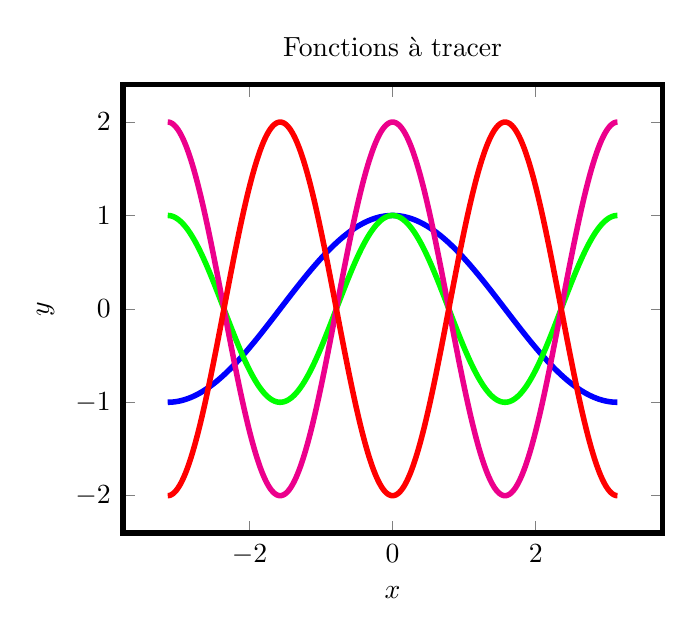
\begin{tikzpicture}
	  \begin{axis}[line width=2pt,       legend columns=-1,
   title=Fonctions à tracer,
   xlabel={$x$},
   ylabel={$y$}, legend entries={$\tr{cos}(x)$,$\tr{cos}(2x)$,$2\cos(-2x)$,$-2\cos(2x)$},
	  legend to name=named]
		\addplot[blue] expression[domain=-pi:pi,samples=500]{cos(180*x/pi)};
		\addplot[green,samples=500] expression[domain=-pi:pi]{cos(2*180*x/pi)};
		\addplot[magenta,samples=500] expression[domain=-pi:pi]{2*cos(2*180*x/pi)};
		\addplot[red,samples=500] expression[domain=-pi:pi]{-2*cos(2*180*x/pi)};				
	  \end{axis}

	\end{tikzpicture}
		  \ref{named}
\end{center}
}